\section{Ejercicio 1: Escribiendo consultas con el operador PIVOT} 
\textbf{}\\
\textbf{Tarea 1: Escriba una declaración SELECT para recuperar el número de clientes para un específico grupo de clientes}
\textbf{}\\
\textbf{}\\
Paso 1. Inicie SQL Server Management Studio y conéctese al motor de base de datos (local) usando Windows autenticación.

\begin{flushleft}

\begin{center}
	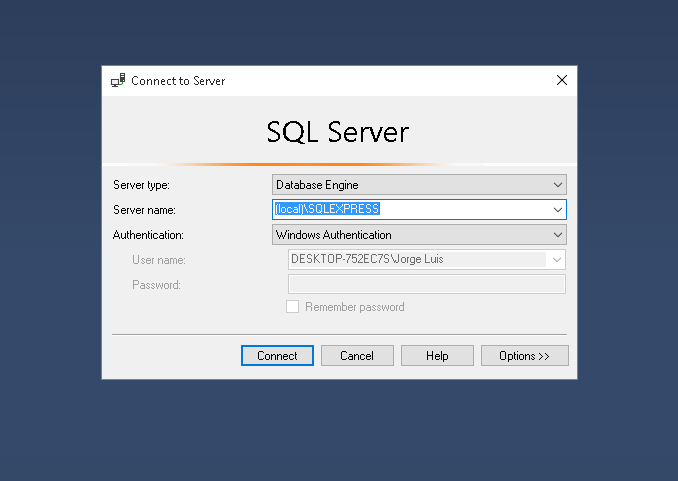
\includegraphics[width=10cm]{./Imagenes/img1} 
	\end{center}


Paso 2. En el menú Archivo, haga clic en Abrir y haga clic en Proyecto / Solución.

\begin{center}
	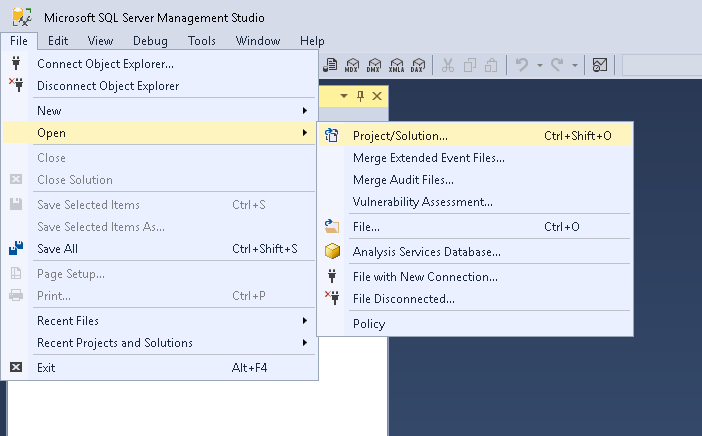
\includegraphics[width=10cm]{./Imagenes/img2} 
	\end{center}

\textbf{}\\
\textbf{}\\
\textbf{}\\
\textbf{}\\
\textbf{}\\
\textbf{}\\
\textbf{}\\
\textbf{}\\
\textbf{}\\
Paso 3. En la ventana Abrir proyecto, abra el proyecto Proyecto.ssmssln.
\begin{center}
	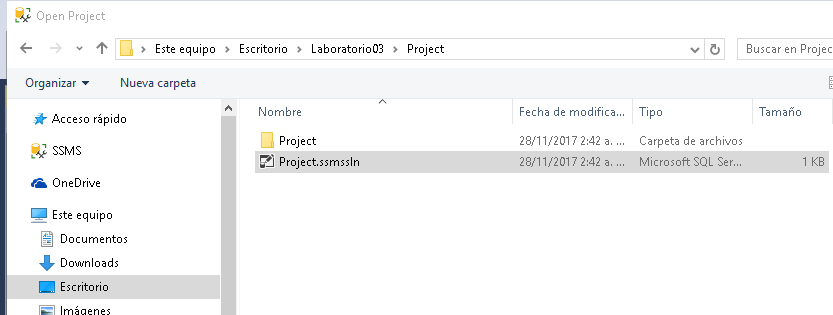
\includegraphics[width=10cm]{./Imagenes/img3} 
	\end{center}

Paso 4. En el Explorador de soluciones, haga doble clic en la consulta 51 - Ejercicio de laboratorio 1.sql.
\begin{center}
	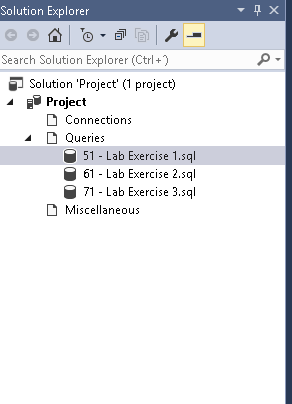
\includegraphics[width=10cm]{./Imagenes/img4} 
	\end{center}
\textbf{}\\
\textbf{}\\
\textbf{}\\

\textbf{}\\
\textbf{}\\
Paso 5. En la ventana de consulta, resalte la instrucción USE TSQL; y haga clic en Ejecutar.
\begin{center}
	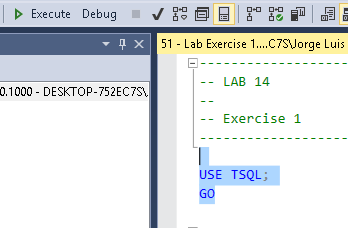
\includegraphics[width=10cm]{./Imagenes/img5} 
	\end{center}

Paso 6. Resalte el siguiente código T-SQL proporcionado:

\begin{center}
	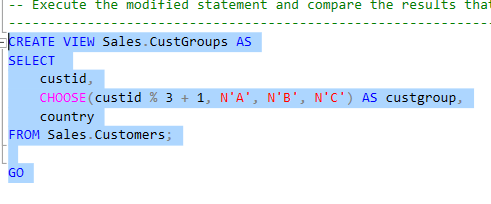
\includegraphics[width=10cm]{./Imagenes/img6} 
	\end{center}

Paso 7. Haga clic en Ejecutar. Este código crea una vista llamada Sales.CustGroups
\begin{center}
	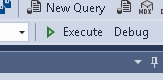
\includegraphics[width=10cm]{./Imagenes/img7} 
	\end{center}
\begin{center}
	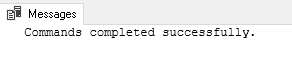
\includegraphics[width=10cm]{./Imagenes/img71} 
	\end{center}

Paso 8. En el panel de consulta, escriba la siguiente consulta después del código T-SQL proporcionado:
\textbf{}\\
\textbf{}\\
SELECT\\
custid,\\
custgroup,\\
country\\
FROM Sales.CustGroups;\\

\textbf{}\\
Paso 9. Resalte la consulta escrita y haga clic en Ejecutar.
\begin{center}
	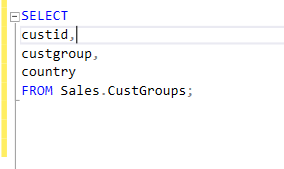
\includegraphics[width=5cm]{./Imagenes/img9} 
	\end{center}
\begin{center}
	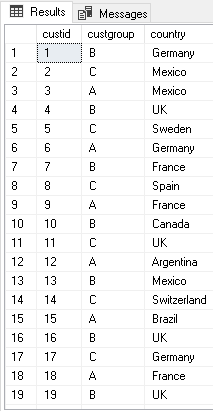
\includegraphics[width=5cm]{./Imagenes/img91} 
	\end{center}


Paso 10. Modifique el código T-SQL escrito aplicando el operador PIVOT. La consulta debería verse así:
\textbf{}\\
\textbf{}\\
SELECT\\
country,\\
p.A,\\
p.B,\\
p.C\\
FROM Sales.CustGroups\\
PIVOT (COUNT(custid) FOR custgroup IN (A, B, C)) AS p;\\

Paso 11. Resalte la consulta escrita y haga clic en Ejecutar.
\textbf{}\\
\begin{center}
	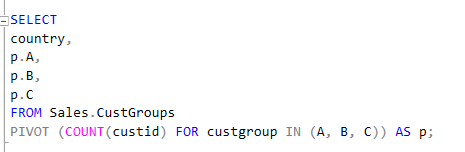
\includegraphics[width=8cm]{./Imagenes/img11} 
	\end{center}
\begin{center}
	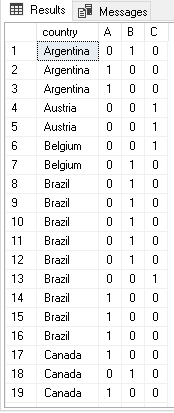
\includegraphics[width=5cm]{./Imagenes/img111} 
	\end{center}

\textbf{Tarea 2: Especifique el elemento de agrupación para el operador PIVOT}
\textbf{}\\
\textbf{}\\
Paso 1. Resalte el siguiente código T-SQL proporcionado después de la descripción de la Tarea 2:
\begin{center}
	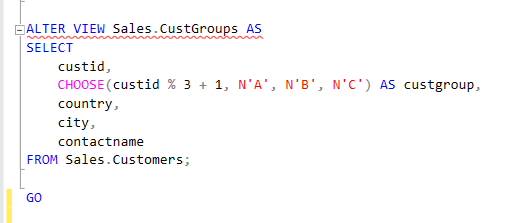
\includegraphics[width=10cm]{./Imagenes/2img1} 
	\end{center}
\textbf{}\\
\textbf{}\\
\textbf{}\\
\textbf{}\\
Paso 2. Haga clic en Ejecutar. Este código modifica la vista agregando dos columnas adicionales.
\begin{center}
	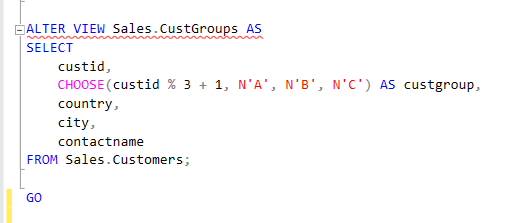
\includegraphics[width=10cm]{./Imagenes/2img1} 
	\end{center}


Paso 3. Resalte la última consulta en la tarea 1. En la barra de herramientas, haga clic en Editar y luego en Copiar
\textbf{}\\
\textbf{}\\
SELECT\\
country,\\
p.A,\\
p.B,\\
p.C\\
FROM Sales.CustGroups\\
PIVOT (COUNT(custid) FOR custgroup IN (A, B, C)) AS p;\\

\textbf{}\\
\textbf{}\\


Paso 4. En la ventana de consulta, haga clic en la línea después del código T-SQL proporcionado. En la barra de herramientas, haga clic en Editar y luego en Pegar.
\begin{center}
	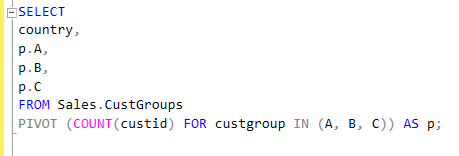
\includegraphics[width=10cm]{./Imagenes/2img4} 
	\end{center}

Paso 5. Resalte la consulta copiada y haga clic en Ejecutar.
\begin{center}
	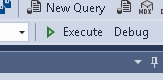
\includegraphics[width=10cm]{./Imagenes/2img5} 
	\end{center}
\textbf{}\\
\textbf{}\\

Paso 6. Observa el resultado. ¿Es este resultado el mismo que el de la consulta en la tarea 1?\\
\textbf{}\\
- El resultado no es el mismo. Más filas fueron devueltas después de que modificó la vista.
\textbf{}\\
\textbf{}\\

Paso 7. Modifique la sentencia T-SQL copiada para incluir columnas adicionales de la vista. La consulta debe se parece a esto:\\
\textbf{}\\
SELECT\\
country,\\
city,\\
contactname,\\
p.A,\\
p.B,\\
p.C\\
FROM Sales.CustGroups\\
PIVOT (COUNT(custid) FOR custgroup IN (A, B, C)) AS p; \\
\textbf{}\\
\textbf{}\\
Paso 8. Resalte la consulta escrita y haga clic en Ejecutar.
\begin{center}
	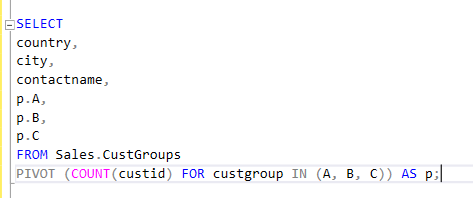
\includegraphics[width=10cm]{./Imagenes/2img8} 
	\end{center}

\begin{center}
	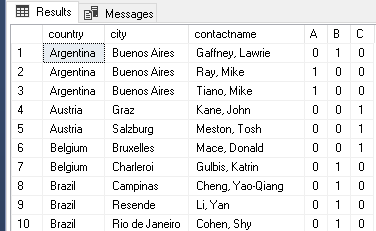
\includegraphics[width=10cm]{./Imagenes/2img81} 
	\end{center}
\textbf{}\\
\textbf{}\\
Paso 9. Observe que recibió el mismo resultado que la consulta anterior. ¿Por qué obtuviste el mismo número de filas?\\
- El operador PIVOT asume que todas las columnas, excepto la agregación y la propagación
Los elementos forman parte de las columnas de agrupación.


\textbf{Tarea 3: usar una expresión de tabla común (CTE) para especificar el elemento de agrupación para el operador PIVOT}
\textbf{}\\
\textbf{}\\

Paso 1. En el panel de consulta, escriba la siguiente consulta después de la descripción de la Tarea 3:
\textbf{}\\
\textbf{}\\
WITH PivotCustGroups AS\\
(\\
SELECT\\
custid,\\
country,\\
custgroup\\
FROM Sales.CustGroups\\
)\\
SELECT\\
country,\\
p.A,\\
p.B,\\
p.C\\
FROM PivotCustGroups\\
PIVOT (COUNT(custid) FOR custgroup IN (A, B, C)) AS p;\\
\textbf{}\\
\textbf{}\\
Paso 2. Resalte la consulta escrita y haga clic en Ejecutar
\begin{center}
	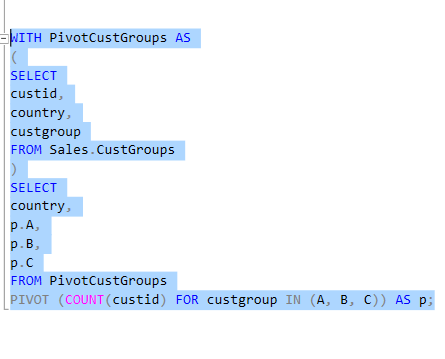
\includegraphics[width=10cm]{./Imagenes/3img1} 
	\end{center}

\textbf{}\\
\textbf{}\\
\textbf{}\\
\textbf{}\\
\textbf{}\\
\textbf{}\\
Paso 3. Observa el resultado. ¿Es el mismo que el resultado de la última consulta en la tarea 1? ¿Puedes explicar por qué? \\
\textbf{}\\
- El resultado es el mismo. En esta tarea, el CTE ha proporcionado tres columnas posibles al operador PIVOT. En tarea 1, la vista también proporcionó tres columnas al operador PIVOT.
\textbf{}\\
\begin{center}
	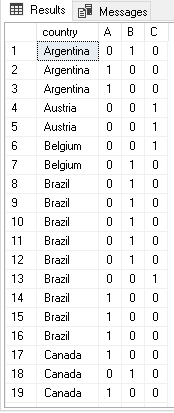
\includegraphics[width=4cm]{./Imagenes/3img3} 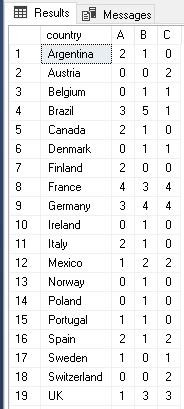
\includegraphics[width=4cm]{./Imagenes/3img31} 
	\end{center}

Paso 4. ¿Por qué cree que es beneficioso utilizar un CTE cuando se usa el operador PIVOT? \\
\textbf{}\\
Al usar el operador PIVOT, usted no puede especificar directamente el elemento de agrupación porque SQL Server automáticamente asume que todas las columnas deben usarse como elementos de agrupación, con la excepción de la propagación y elementos de agregación. Con un CTE, puede especificar las columnas exactas y, por lo tanto, controlar que Columnas utilizadas para la agrupación.
\textbf{}\\
\textbf{}\\
\textbf{}\\
\textbf{}\\
\textbf{}\\
\textbf{}\\

\textbf{}\\
\textbf{}\\
\textbf{}\\
\textbf{}\\
\textbf{}\\
\textbf{Tarea 4: Escriba una instrucción SELECT para recuperar el monto total de ventas para cada uno de Categoría de cliente y producto}
\textbf{}\\
\textbf{}\\

Paso 1. En el panel de consulta, escriba la siguiente consulta después de la descripción de la Tarea 4.
\textbf{}\\
\textbf{}\\
\begin{center}
	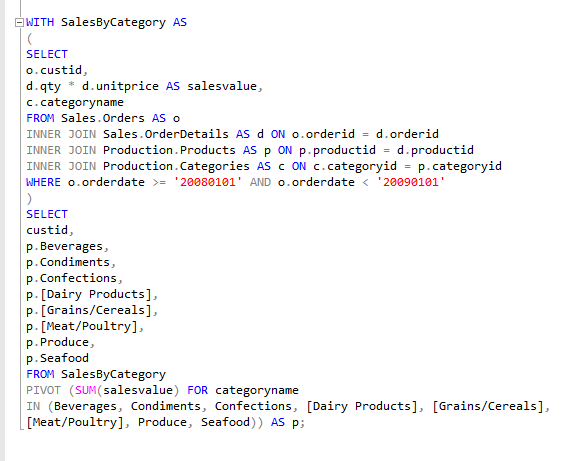
\includegraphics[width=10cm]{./Imagenes/4img1}
	\end{center}
\textbf{}\\
\textbf{}\\
Paso 2. Resalte la consulta escrita y haga clic en Ejecutar.
\textbf{}\\
\textbf{}\\
\begin{center}
	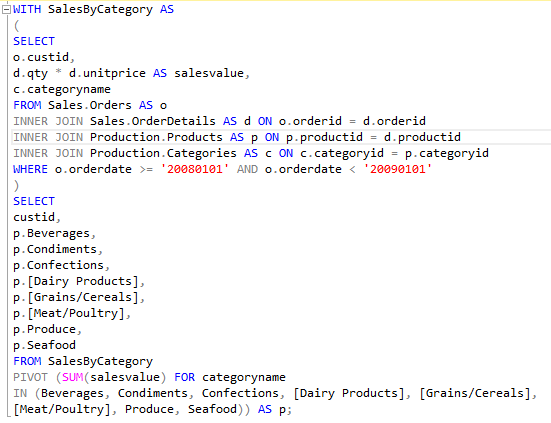
\includegraphics[width=10cm]{./Imagenes/4img2}
	\end{center}
\textbf{}\\
\textbf{}\\
\begin{center}
	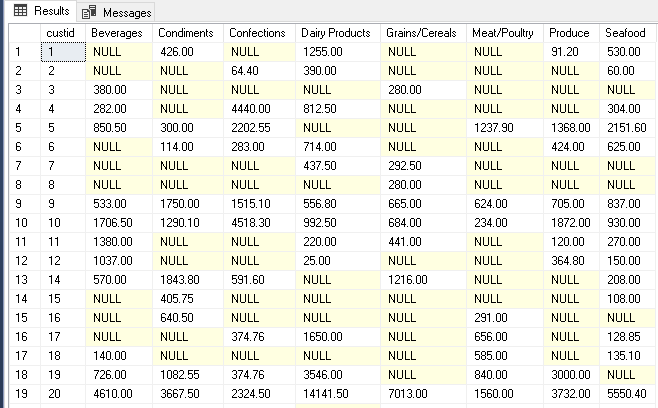
\includegraphics[width=10cm]{./Imagenes/4img3}
	\end{center}








\end{flushleft}